\documentclass[border=10pt]{standalone}

\usepackage{tikz}
\usepackage{tikzsymbols}
\usetikzlibrary{calc,patterns,shapes.geometric}

\def\centerarc[#1](#2)(#3:#4:#5){\draw[#1] ($(#2)+({#5*cos(#3)},{#5*sin(#3)})$) arc (#3:#4:#5);}

\begin{document}
	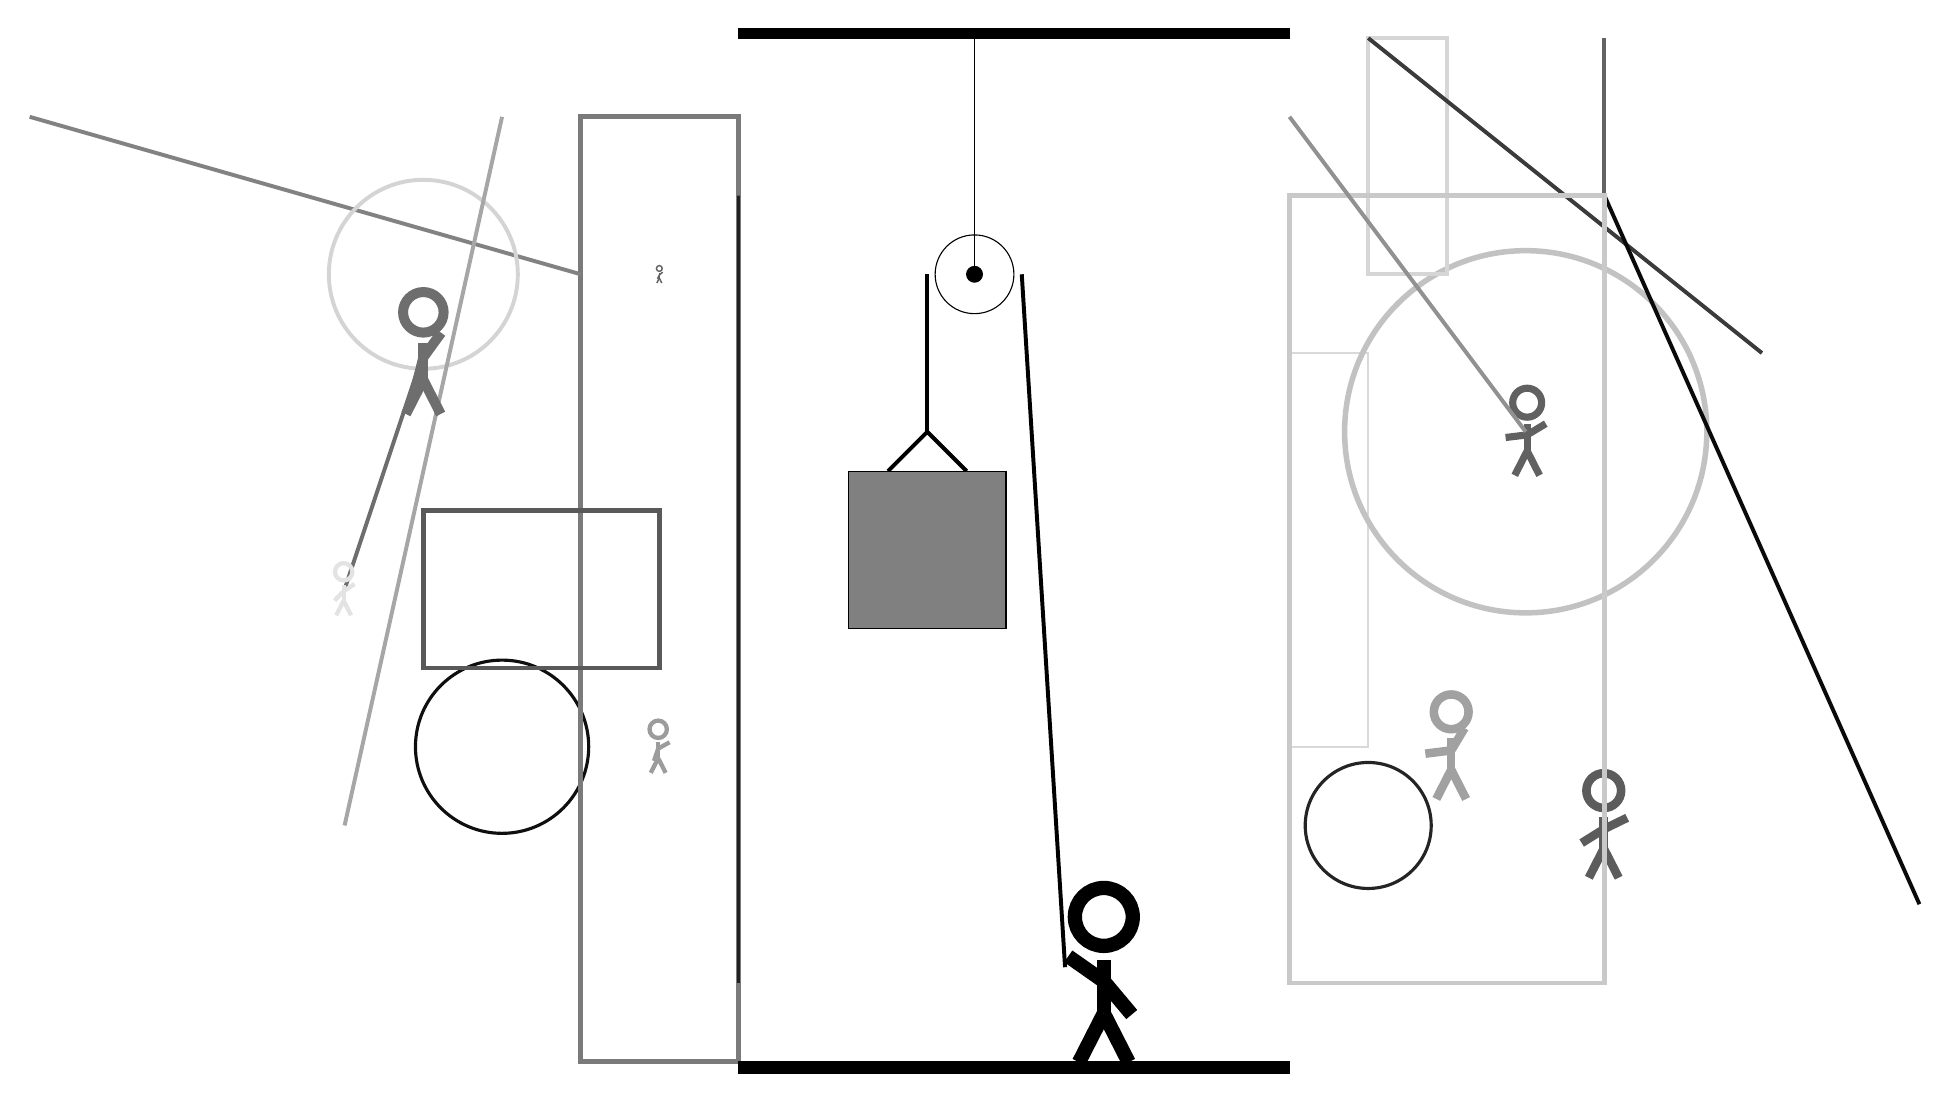
\begin{tikzpicture}
		%%%%% START %%%%%
		
		\draw[fill=black] (-2, 10) rectangle (5, 10.125);
		
		\node[line width=0.2mm, color=black!62] at (-3, 7) {\Strichmaxerl[1][65][39]};
		
		\draw[line width=0.3mm, color=black!15] (5, 6) rectangle (6, 1);
		\draw [line width=0.7mm, color=black!24](8, 5) circle (2.3);
		\draw [line width=0.4mm, color=black!94](-5, 1) circle (1.1);
		\draw[line width=0.5mm, color=black!16] (7, 10) rectangle (6, 7);
		
		\draw[line width=0.6mm, color=black!52] (-4, -3) rectangle (-2, 9);
		\draw[line width=0.5mm, color=black!77](6, 10) -- (11, 6);
		\draw[line width=0.5mm, color=black!96](9, 8) -- (13, -1);
		\draw[line width=0.4mm, color=black!87] (-2, -2) rectangle (-2, 8);
		
		\draw[line width=0.5mm, color=black!49](-4, 7) -- (-11, 9);
		
		\node[line width=0.4mm, color=black!37] at (7, 1) {\Strichmaxerl[6][7][59]};
		\draw[line width=0.6mm, color=black!65] (-3, 2) rectangle (-6, 4);
		\node[line width=0.3mm, color=black!64] at (9, 0) {\Strichmaxerl[6][32][26]};
		\node[line width=0.3mm, color=black!62] at (8, 5) {\Strichmaxerl[5][7][31]};
		\draw[line width=0.5mm, color=black!61](9, 10) -- (9, 8);
		\node[line width=0.3mm, color=black!39] at (-3, 1) {\Strichmaxerl[3][71][29]};
		
		\draw [line width=0.5mm, color=black!17](-6, 7) circle (1.2);
		\draw[line width=0.6mm, color=black!21] (5, -2) rectangle (9, 8);
		\draw[line width=0.5mm, color=black!35](-7, 0) -- (-5, 9);
		\draw[line width=0.5mm, color=black!57](-6, 6) -- (-7, 3);
		\draw [line width=0.4mm, color=black!86](6, 0) circle (0.8);
		\node[line width=0.6mm, color=black!57] at (-6, 6) {\Strichmaxerl[7][76][54]};
		\draw[line width=0.5mm, color=black!43](5, 9) -- (8, 5);
		\node[line width=0.7mm, color=black!11] at (-7, 3) {\Strichmaxerl[3][46][33]};
		
		\draw (1, 7) circle (0.5);
		\draw[fill=black] (1, 7) circle (0.1);
		\draw (1, 10) -- (1, 7);
		
		\draw[line width=0.5mm] (-0.1, 4.5) -- (0.4, 5.0) -- (0.9, 4.5);
		\draw[fill=black!50] (-0.6, 4.5) rectangle (1.4, 2.5);
		
		\draw[line width=0.5mm] (0.4, 7) -- (0.4, 5.0);
		\centerarc[line width=0.5mm](1, 7)(0:180:0.6);
		\draw[line width=0.5mm](1.6, 7) -- (2.15, -1.8);
		
		\node at (2.6, -1.9) {\Strichmaxerl[10][-35][-50]};
		
		\draw[fill=black] (-2, -3) rectangle (5, -3.15);
		
		%%%%% END %%%%%
	\end{tikzpicture}
\end{document}